\documentclass[
	a4paper,
	oneside,
	% BCOR = 10mm,
	DIV = 12,
	fontsize = 13pt,
	headings = normal,
	numbers = endperiod,
	bibliography = totoc, % place bibliography in toc without a number
]{scrartcl}

%%% Length calculations
\usepackage{calc}
%%%

%%% Support for color
\usepackage{xcolor}
\definecolor{lightblue}{HTML}{03A9F4}
\definecolor{red}{HTML}{F44336}
%%%

%%% Including graphics
\usepackage{graphicx}
%%%

%%% Font selection
\usepackage{fontspec}

\setromanfont{STIX Two Text}[
	Path              = {./fonts/},
	UprightFont       = {STIX2Text-Regular.otf},
	ItalicFont        = {STIX2Text-Italic.otf},
	BoldFont          = {STIX2Text-Bold.otf},
	BoldItalicFont    = {STIX2Text-BoldItalic.otf},
	SmallCapsFeatures = {LetterSpace = 8},
]

\setsansfont{IBM Plex Sans}[
	Path              = {./fonts/},
	UprightFont       = {IBMPlexSans-Regular.otf},
	ItalicFont        = {IBMPlexSans-Italic.otf},
	BoldFont          = {IBMPlexSans-Bold.otf},
	BoldItalicFont    = {IBMPlexSans-BoldItalic.otf},
	Scale = MatchUppercase,
]

\setmonofont{IBM Plex Mono}[
	Path              = {./fonts/},
	UprightFont       = {IBMPlexMono-Regular.otf},
	ItalicFont        = {IBMPlexMono-Italic.otf},
	BoldFont          = {IBMPlexMono-Bold.otf},
	BoldItalicFont    = {IBMPlexMono-BoldItalic.otf},
	Scale = MatchUppercase,
]
%%%

%%% Math typesetting
\usepackage{amsmath}

\usepackage{amsthm}
\newtheoremstyle{mythm}%
	{1\baselineskip} % Space above
	{1\baselineskip} % Space below
	{\upshape} % Body font
	{} % Indent amount
	{\upshape\bfseries} % Theorem head font
	{.} % Punctuation after theorem head
	{0.5em} % Space after theorem head
	{} % Theorem head spec
\theoremstyle{mythm}
\newtheorem{mythm}{Теорема}
\newtheorem{mydef}{Визначення}

\usepackage{IEEEtrantools}

\usepackage{unicode-math}
\setmathfont{STIX Two Math}
%%%

%%% List settings
\usepackage{enumitem}
\setlist[enumerate]{
	label*      = {\arabic*.},
	leftmargin  = *,
	labelindent = \parindent,
	topsep      = 1\baselineskip,
	parsep      = 0\baselineskip,
	itemsep     = 1\baselineskip,
	noitemsep,
}

\setlist[itemize]{
	label*      = {—},
	leftmargin  = *,
	% labelindent = \parindent,
	align       = left,
	topsep      = 1\baselineskip,
	parsep      = 0\baselineskip,
	itemsep     = 0\baselineskip,
}

\setlist[description]{
	font        = {\rmfamily\upshape\bfseries},
	topsep      = 1\baselineskip,
	parsep      = 0\baselineskip,
	itemsep     = 0\baselineskip,
}

\newlist{termpaperinfo}{enumerate}{3}
\setlist[termpaperinfo]{
	label*      = {\arabic*.},
	leftmargin  = *,
	align       = left,
	topsep      = 1\baselineskip,
	parsep      = 0\baselineskip,
	itemsep     = 1\baselineskip,
}

%%%

%%% Structural elements typesetting
\setkomafont{pagenumber}{\rmfamily\upshape}
\setkomafont{disposition}{\rmfamily\bfseries}

% Sectioning
\RedeclareSectionCommand[
	beforeskip = -1\baselineskip,
	afterskip  = 1\baselineskip,
	font       = {\normalsize\bfseries},
]{section}

% \renewcommand*{\sectionformat}{\thesection\autodot\enskip}

\renewcommand{\sectionlinesformat}[4]{%
	\centering{}#3#4%
}

\RedeclareSectionCommand[
	beforeskip = -1\baselineskip,
	afterskip  = 1\baselineskip,
	font       = {\normalsize\bfseries},
]{subsection}

\RedeclareSectionCommand[
	beforeskip = -1\baselineskip,
	afterskip  = 1\baselineskip,
	font       = {\normalsize\bfseries},
]{subsubsection}

\RedeclareSectionCommand[
	beforeskip = -1\baselineskip,
	afterskip  = -0.5em,
	font       = {\normalsize\mdseries\scshape\addfontfeatures{Letters = {UppercaseSmallCaps}}},
]{paragraph}

\DeclareNewSectionCommand[
	style = section,
	afterskip = 1\baselineskip,
	beforeskip = -1\baselineskip,
	font = \usekomafont{section},
	indent = 0pt,
	level = 1,
	tocindent = 0em,
	toclevel = 1,
	tocnumwidth = 6em,
	tocstyle = section,
	% indent=0pt,
	% beforeskip=-3.5ex plus -1ex minus -.2ex,
	% afterskip=2.3ex plus .2ex,
	% tocindent=1.5em,
	% tocnumwidth=7em,
	% counterwithin=chapter,
]{appsection}

\makeatletter
\AtBeginDocument{\let\toclevel@subappendix\toclevel@section}
\makeatother

\renewcommand\theappsection{\Alph{appsection}}
\renewcommand\appsectionformat{\appendixname~\theappsection\autodot\enskip}
\renewcommand\addappsectiontocentry[2]{%
		\addtocentrydefault{appsection}{\appendixname~#1}{#2}%
}

%%%

%%% Typographic enhancements
\usepackage{microtype}
%%%

%%% Language-specific settings
\usepackage{polyglossia}
\setmainlanguage{ukrainian}
\setotherlanguages{english}
%%%

%%% Captions
\usepackage{caption}
\usepackage{subcaption}

%\DeclareCaptionLabelFormat{closing}{#2)}
%\captionsetup[subtable]{labelformat = closing}

%\captionsetup[subfigure]{labelformat = closing}

\captionsetup[table]{
	aboveskip = 0\baselineskip,
	belowskip = 0\baselineskip,
}

\captionsetup[figure]{
	aboveskip = 1\baselineskip,
	belowskip = 0\baselineskip,
}

\captionsetup[subfigure]{
	labelformat = simple,
	labelformat = brace,
}
%%%

%%% Change counters
\usepackage{chngcntr}
\counterwithin{equation}{section}
%%%

%%% Hyphenated ragged typesetting
\usepackage{ragged2e}
%%%

%%% Table typesetting
\usepackage{booktabs}
\usepackage{longtable}

\usepackage{multirow}

\usepackage{array}
\newcolumntype{v}[1]{>{\RaggedRight\arraybackslash\hspace{0pt}}p{#1}}
\newcolumntype{b}[1]{>{\Centering\arraybackslash\hspace{0pt}}p{#1}}
\newcolumntype{n}[1]{>{\RaggedLeft\arraybackslash\hspace{0pt}}p{#1}}
%%%

%%% Drawing
\usepackage{tikz}
\usepackage{tikzscale}
\usetikzlibrary{positioning}
\usetikzlibrary{arrows.meta} % Stealth arrow tips
\usetikzlibrary{shapes.multipart}
\usetikzlibrary{decorations.pathreplacing}
%%%

%%% SI units typesetting
\usepackage{siunitx}
\sisetup{
	output-decimal-marker = {,},
	exponent-product      = {\cdot},
	inter-unit-product    = \ensuremath{{} \cdot {}},
	per-mode              = symbol,
}
%%%

%%% Code highlighting
\usepackage{minted}

\newmintinline[pyinline]{python}{
	style = bw,
	breaklines,
	% breakbytokenanywhere,
	breakafter = { _},
	breakaftersymbolpre = {\textrm{-}},
}

\newminted{bash}{
	linenos,
	style = bw,
	breaklines,
	breakbytokenanywhere,
	autogobble, % automatically determine how many characters to gobble
}
%%%

%%% Framing code listings
\usepackage{tcolorbox}
\tcbuselibrary{breakable}
\tcbuselibrary{minted}
\tcbuselibrary{skins}

\newtcblisting[auto counter, list inside, number within = section]{listingpython}[3][]{%
	minted language = python,
	minted style    = bw,
	minted options  = {
		linenos,
		tabsize = 4,
		breaklines,
		% breakanywhere,
		fontsize = \footnotesize,
		autogobble
	},
	%
	% empty,
	sharp corners,
	colframe         = black,
	colback          = black!0,
	leftrule         = 0em,
	rightrule        = 0em,
	toprule          = 1pt, % orig = 0pt
	bottomrule       = 1pt, % orig = 0pt
	titlerule        = 0.5pt,
	colbacktitle     = black!0,
	coltitle         = black,
	toptitle         = 0.3em,
	bottomtitle      = 0.1em,
	borderline north = {1pt}{0pt}{black},
	borderline south = {1pt}{0pt}{black},
	before skip      = \intextsep,
	after  skip      = \intextsep,
	title            = {Лістинг \thetcbcounter: #2},
	list entry       = {\protect\numberline{\thetcbcounter}#2},
	left = 0em,
	right = 0em,
	%
	listing only,
	breakable,
	%
	label = {#3},
	%
	#1
}

\newtcbinputlisting[auto counter, list inside, number within = section]{\inputpython}[4][]{%
	minted language = python,
	minted style    = bw,
	minted options  = {
		linenos,
		tabsize = 4,
		breaklines,
		breakbytokenanywhere,
		fontsize = \footnotesize,
	},
	%
	% empty,
	sharp corners,
	colframe         = black,
	colback          = black!0,
	leftrule         = 0em,
	rightrule        = 0em,
	toprule          = 0pt, % orig = 0pt
	bottomrule       = 0pt, % orig = 0pt
	titlerule        = 0.5pt,
	colbacktitle     = black!0,
	coltitle         = black,
	toptitle         = 0.3em,
	bottomtitle      = 0.1em,
	borderline north = {1pt}{0pt}{black},
	borderline south = {1pt}{0pt}{black},
	before skip      = \intextsep,
	after  skip      = \intextsep,
	title            = {Лістинг \thetcbcounter: #3},
	list entry       = {\protect\numberline{\thetcbcounter}#3},
	left = 0em,
	right = 0em,
	%
	listing file={#2},
	listing only,
	breakable,
	%
	label = {#4},
	%
	#1
}

% Customize minted line numbers
\renewcommand{\theFancyVerbLine}{\ttfamily\scriptsize\arabic{FancyVerbLine}}

%%%

%%% Bibliography
\usepackage[
	style    = gost-numeric,
	language = auto,
	autolang = other,
	sorting  = none,
]{biblatex}
\addbibresource{y03s01-syssoft-term-paper-01-bibliography.bib}
%%%

%%% Links and hyperreferences
\usepackage{hyperref}
\hypersetup{
	bookmarksnumbered = true,
	colorlinks      = false,
	linkbordercolor = red,
	urlbordercolor  = lightblue,
	pdfborderstyle  = {/S/U/W 1.5},
}
%%%

%%% Length adjustments
% Set baselineskip, default is 14.5 pt
\linespread{1.068966} % ~15.5 pt
\setlength{\emergencystretch}{1em}
\setlength{\parindent}{1.5em}
\newlength{\gridunitwidth}
\setlength{\gridunitwidth}{\textwidth / 12}
%%%

%%% Custom commands
\newcommand{\blankspace}[1]{\underline{\hspace{#1}}}
\newcommand{\allcaps}[1]{{\addfontfeatures{LetterSpace = 8, Kerning = Off}#1}}
\newcommand{\filename}[1]{\texttt{#1}}
\newcommand{\progname}[1]{\texttt{#1}}
\newcommand{\modulename}[1]{\texttt{#1}}

\newcommand{\myvec}[1]{\mathbf{#1}}
%%%

%%% Custom math commands
\DeclareMathOperator{\classify}{classify}
\DeclareMathOperator{\zip}{zip}
\DeclareMathOperator*{\argmax}{arg\,max} % starred to place subsctipt below function name in display style
\DeclareMathOperator*{\argmin}{arg\,min} % starred to place subsctipt below function name in display style

\newcommand{\longvar}[1]{\mathit{#1}}
%%%

\begin{document}

\begin{titlepage}
		\begin{center}
			Міністерство освіти і науки України\\
			Національний авіаційний університет\\
			Навчально-науковий інститут комп'ютерних інформаційних технологій\\
			Кафедра комп'ютеризованих систем управління

			\vspace{\fill}
				Курсова робота\\
				з дисципліни «Системне програмне забезпечення»\\

				\vspace*{3\baselineskip}

				Пояснювальна записка\\
				Тема: реалізація наївного баєсового класифікатора на~мові~програмування~\textenglish{Python}

			\vspace{\fill}

			\begin{flushright}
				Виконав:\\
				студент групи СП-325\\
				Клокун В.\,Д.\\
			\end{flushright}

			Київ — 2018
		\end{center}
	\end{titlepage}

	\section*{Завдання на~виконання курсової~роботи\\студента групи~СП-325 Клокуна Владислава~Денисовича}
	% {\centering{}студента групи~СП-325 Клокуна Владислава Денисовича\par}
	\begin{termpaperinfo}
		\item Тема курсової роботи: реалізація наївного баєсового класифікатора на~мові~програмування~\textenglish{Python} для класифікації спостережень, що~містять неперервні числові дані.
		\item Термін виконання курсової роботи:\\ з~«\blankspace{1cm}» \blankspace{4cm}~2018~р. по~«\blankspace{1cm}»~\blankspace{4cm}~2018~р.
		\item Вхідні дані до роботи: набір даних для класифікації.
		\item Етапи виконання курсової роботи:
			\begin{itemize}
				\item Огляд теоретичних відомостей про наївний баєсів класифікатор.
				\item Постановка задачі.
				\item Реалізація наївного баєсового класифікатора.
				\item Тестування розробленої реалізації наївного баєсового класифікатора.
			\end{itemize}
		\item Перелік обов'язкових додатків і графічного матеріалу:
			\begin{itemize}
				\item Початковий код розробленої реалізації.
				\item Зміст набору вхідних даних~«Іриси Фішера».
			\end{itemize}
	\end{termpaperinfo}

	{%
		\newlength{\blanklinematch}
		\setlength{\blanklinematch}{1cm + \widthof{» } + 5cm}
		\noindent%
		\begin{tabular}{
				@{}ll
			}
			Завдання отримав: & «\blankspace{1cm}» \blankspace{5cm}~2018~р.\\
			Підпис студента:  & \phantom{«}\blankspace{\blanklinematch}~(Клокун В.\,Д.)\\
			% Підпис студента:  & \blankspace{\widthof{«} + 1cm + \widthof{»} + 5cm}~(Клокун В.\,Д.)
		\end{tabular}
		\par
	}

	\newpage
	\tableofcontents

	\newpage
	\section{Теоретична частина}
		\subsection{Загальна характеристика наївного баєсового класифікатора}
			\label{ssec:theory-short}
			Припустимо, що~в~ході деякого експерименту проводились спостереження, під час проведення яких збирались неперервні (недискретні) дані про~результат події. Також були визначені категорії (або класи), до~яких ці~дані можуть належати. Поставлена задача класифікувати дані спостережень. \emph{Класифікація}~— це~задача визначення, до~якої з~категорій належить певне спостереження.~\cite{wiki-stat-classification} \emph{Класифікатор}~— це~алгоритм, який виконує класифікацію.~\cite{wiki-stat-classification}

			\emph{Наївний баєсів класифікатор}~— це ймовірнісний класифікатор, який використовує теорему Баєса для класифікації спостережень. Такі класифікатори отримують на вхід спостереження, оцінюють його і~роблять припущення про~клас, до~якого воно~належить. Вхідні дані, тобто спостереження, представляються у~вигляді вектора відомих значень випадкових змінних, які називаються \emph{ознаками}. Результатом роботи класифікатора є~певне значення цільової змінної або змінних, які зазвичай називаються класовими, і позначають клас, до~якого належить спостереження.

			Принцип класифікації полягає в~обчисленні умовних імовірностей~(визначення~\ref{def:conditional-probability}) того, що~вхідні дані належать до~певних класів~(події, які~нас цікавлять), за~умови, що~ознаки мають певні значення~(події, які ми спостерігаємо). Після обчислення кожної з~умовних імовірностей за~обраним правилом прийняття рішення~робиться висновок, до якого класу належить задане спостереження. Оскільки такий класифікатор використовує ймовірнісну модель, наївний баєсів класифікатор називають~\emph{імовірнісним}.

			\begin{mydef}[Умовна ймовірність]
				\label{def:conditional-probability}
				Нехай~$A$ і~$B$~— події. Позначимо ймовірність настання кожної з~них незалежно одна від~одної як~$P(A)$ і~$P(B)$ відповідно. Тоді \emph{умовною імовірністю}~$P(A \mid B)$ називається ймовірність настання події~$A$ за~умови, що~подія~$B$ настала. Вона обчислюється так:
				\begin{IEEEeqnarray}{rCl}
					P(A \mid B) = \frac{P(A \cap B)}{P(B)},
				\end{IEEEeqnarray}
				де~$P(A \cap B)$~— ймовірність, що події~$A$ і~$B$ настали. 
			\end{mydef}
			
			Розглянемо приклад класифікації наївним баєсовим класифікатором. Нехай подія~$A$~— дане спостереження належить до~певного класу, подія~$B$~— ознаки спостереження мають певні значення. Тоді щоб знайти ймовірність, що дане спостереження з~певним значенням ознак належить до~певного класу, необхідно обчислити умовну ймовірність~$P(A \mid B)$. Для~обчислення цієї імовірності необхідно використати теорему~Баєса~(теорема~\ref{thm:theorem-bayes}).

			\begin{mythm}[Баєса]
				\label{thm:theorem-bayes}
				Нехай~$P(A \mid B)$~— умовна ймовірність настання події~$A$ за~умови, що~подія~$B$ настала, $P(B \mid A)$~— умовна ймовірність настання події~$B$ за~умови, що~подія~$A$ настала; $P(B)$~— імовірність настання події~$B$, причому~$P(B) \neq 0$. Тоді умовна ймовірність~$P(A \mid B)$ обчислюється так:
				\begin{IEEEeqnarray}{rCl}
					P(A \mid B) = \frac{P(B \mid A) \, P(A)}{P(B)}.
				\end{IEEEeqnarray}
			\end{mythm}

			\begin{proof}
				Виразимо ймовірності~$P(A \mid B)$ і~$P(B \mid A)$ за~визначенням умовної ймовірності:
				\begin{IEEEeqnarray}{rCl}
					\label{eq:p-ab}
					P(A \mid B) &=& \frac{P(A \cap B)}{P(B)},\, P(B) \neq 0,\\ \IEEEstrut[4\jot]
					\label{eq:p-ba}
					P(B \mid A) &=& \frac{P(B \cap A)}{P(A)},\, P(A) \neq 0.
				\end{IEEEeqnarray}
				Представимо ймовірності настання подій~$A$ і~$B$ разом, тобто~$P(A \cap B)$ і~$P(B \cap A)$ з~\eqref{eq:p-ab}, \eqref{eq:p-ba}:
				\begin{IEEEeqnarray}{rCl}
					P(A \cap B) &=& P(A \mid B) \, P(B),\\
					P(B \cap A) &=& P(B \mid A) \, P(A).
				\end{IEEEeqnarray}
				Оскільки ліві частини рівні за аксіомою~$P(A \cap B) = P(B \cap A)$, то і~праві частини також будуть рівними: $P(A \mid B) \, P(B) = P(B \mid A) \, P(A)$, отже можна записати, що:
				\begin{IEEEeqnarray}{rCl+x*}
					\label{eq:pab-eq-pba-pb}
					P(A \cap B) = P(B \mid A) \, P(A).
				\end{IEEEeqnarray}
				Підставимо~\eqref{eq:pab-eq-pba-pb} в~\eqref{eq:p-ab} і~отримаємо:
				\begin{IEEEeqnarray}{rCl+x*}
					P(A \mid B) &=& \frac{P(A \cap B)}{P(B)} = \frac{P(B \mid A) \, P(A)}{P(B)},\, P(B) \neq 0.
					\\* &&& \qedhere\nonumber
				\end{IEEEeqnarray}
			\end{proof}

			Як видно, при~класифікації наївним баєсовим класифікатором, у~обчисленні умовних імовірностей використовується теорема Баєса, тому~такий імовірнісний класифікатор називається \emph{баєсовим}.

		\subsection{Імовірнісна модель наївного баєсового класифікатора}
			Як було сказано у~підрозділі~\ref{ssec:theory-short}, наївний баєсів класифікатор використовує ймовірнісну модель. Побудуємо та~представимо~її. Для~виконання класифікації необхідні вхідні дані, тобто спостереження, та~набір можливих значень класової змінної для~позначення класів, до~яких можуть належати ці~дані. Позначатимемо змінні, на~кшталт~$X_i$, великими літерами, а~їх~значення, наприклад, $x_i$~— малими. Вектори, на~зразок~$\myvec{X}$~— жирним шрифтом.
			
			Вхідними даними для~класифікації буде вектор ознак~$\myvec{X} = \left( X_1, \dots, X_n \right)$, де~$X_1, \dots, X_n$~— ознаки. Кожна ознака може мати значення зі~своєї області визначення, яка позначається~$D_i$. Набір усіх векторів ознак позначається як~$\Omega = D_1 \times \dots \times D_n$. Для позначення класу, до якого належить спостереження, введемо випадкову змінну~$C$, де~$C$ може приймати одне з~$m$ значень: $c \in \{ 0, \dots, m - 1\}$. 

			\begin{mydef}[Розподіл імовірностей]
				Нехай~$X$ і~$Y$~— випадкові змінні, які приймають значення~$x$ та~$y$ відповідно. Тоді розподіл імовірностей~$p(X \mid Y)$ позначає значення імовірностей~$P(X = x_i \mid Y = y_i)$ для кожної з можливих пар~$i, j$.~\cite{russel-norvig-ai-ma}
			\end{mydef}

			Класифікація за допомогою наївного баєсового класифікатора ставить у~відповідність кожному вектору~$\myvec{X}$, який~містить ознаки~$X_1, \dots, X_n$, розподіли ймовірностей~$p(C \mid \myvec{X})$. Тобто сама модель має такий загальний вигляд:
			\begin{equation}
				p\left( C \mid \myvec{X} \right) = p\left( C \mid X_1, \dots, X_n \right).
			\end{equation}
			Зі~зростанням кількості або~можливих значень ознак, з~такою моделлю неможливо працювати за~допомогою таблиць імовірностей, тому~переформулюємо модель, щоб~зробити її зручнішою.

			Використовуючи теорему Баєса, представимо її так:
			\begin{equation}
				p(C \mid X_1, \dots, X_n) = \frac{p(C) \, p(X_1, \dots, X_n \mid C)}{p( X_1, \dots, X_n)}.
			\end{equation}
			Видно, що~дільник не~залежить від~змінної~$C$, а~значення ознак~$X_i$ задані наперед, тому на~практиці значення дільника постійне. Ділене рівносильне такій моделі спільного розподілу:
			\begin{equation}
				p(C, X_1, \dots, X_n).
			\end{equation}
			Перетворюємо дану модель за~допомогою визначення умовної ймовірності:
			\begin{IEEEeqnarray}{rCl}
				p(C, X_1, \dots, X_n) &=& p(C) \, p(X_1, \dots, X_n \mid C)\\
				                      &=& p(C) \, p(X_1 \mid C) \, p(X_2, \dots, X_n \mid C, X_1)\\
															&=& p(C) \, p(X_1 \mid C) \, p(X_2 \mid C, X_1) \, p(X_3, \dots, X_n \mid C, X_1, X_2)\: \\
															&=& p(C) \, p(X_1 \mid C) \, p(X_2 \mid C, X_1) \, p(X_3 \mid C, X_1, X_2) \nonumber\\
															&& \> p(X_4, \dots, X_n \mid C, X_1, X_2, X_3)
			\end{IEEEeqnarray}
			і~так далі. Тепер припускаємо, що кожна ознака~$X_i$ умовно незалежна від~кожної іншої ознаки~$X_j$, для будь-яких~$j \neq i$ та~заданої категорії~$C = c$. Математично це означає:
			\begin{IEEEeqnarray*}{rCl}
				p (X_i \mid C, X_j) = p (X_i \mid C).
			\end{IEEEeqnarray*}
			Таке припущення є наївним, оскільки немає жодних підстав вважати, що вхідні ознаки дійсно незалежні одна від одної. Саме тому такий баєсів класифікатор називається \emph{наївним}.

			% \begin{IEEEeqnarray*}{rCl}
			% 	p(C, X_1, \dots, X_n) &=& p( X_1, \dots, X_n, C) \\
			% 												&=& p( X_1 \mid X_2, \dots, X_n, C) \, p(X_2, \dots, X_n, C) \\
			% 												&=& p( X_1 \mid X_2, \dots, X_n, C) \, p( X_2 \mid X_3, \dots, X_n, C) \, p(X_3, \dots, X_n, C) \\
			% 												&\dots& \\
			% 												&=& p( X_1 \mid X_2, \dots, X_n, C) \, p( X_2 \mid X_3, \dots, X_n, C) \dots p(X_{n-1} \mid X_n, C) \, p(X_n | C) \, p(C). \\
			% \end{IEEEeqnarray*}

			Отже, виражаємо загальну модель:
			\begin{IEEEeqnarray}{rCl}
				\label{eq:probability-model-general}
				p(C \mid X_1, \dots, X_n) &=& p(C) \, p(X_1 \mid C) \, p(X_2 \mid C) \dots p(X_n \mid C) \\
																	&=& p(C) \prod_{i=1}^{n} p(X_i \mid C).
			\end{IEEEeqnarray}
			Це означає, що враховуючи припущення про незалежність змінних, умовний розподіл над класовою змінною~$C$ може бути виражений так:
			\begin{IEEEeqnarray}{rCl}
				\label{eq:probability-model-final}
				p(C \mid X_1, \dots, X_n) = \frac{1}{Z} \, p(C) \prod_{i=1}^{n} p( X_i \mid C),
			\end{IEEEeqnarray}
			де~$Z$~— коефіцієнт,~який залежить виключно від~$X_1, \dots, X_n$. Якщо~значення ознак~$x_1, \dots, x_n$ відомі, коефіцієнт~$Z$ сталий.

			Таку модель значно зручніше використовувати, оскільки вони використовують апріорні імовірності класів~$p(C)$ та незалежні розподіли~$p(X_i \mid C)$. Якщо є~$k$~класів та модель модель для~$p(X_i)$ може бути виражена $r$~ параметрами, то відповідний наївний баєсів класифікатор матиме~$(k - 1) + nrk$ параметрів.~\cite{murty-devy-pattern-rec}

		\subsection{Оцінка параметрів}
			Описавши ймовірнісну модель, необхідно визначити її параметри, тобто апріорні ймовірності належності до~класу~$p(C)$ та~розподіли ймовірностей ознак~$p(X_i \mid C)$. Для обчислення параметрів моделі використовують \emph{тренувальний набір даних}~— такий набір даних, який складається із заздалегідь класифікованих спостережень. Тобто набір даних~$S$ складатиметься з~векторів~$\myvec{x} = (x_1, \dots, x_n, c)$, де~$c$~— правильне значення класової змінної.
			
			Усі параметри моделі можна обчислити з~тренувального набору даних.~\cite{murty-devy-pattern-rec} Щоб оцінити значення параметрів, необхідно зробити припущення щодо розподілу, який характеризує дані. Припущення щодо розподілу, який характеризує дані, називають \emph{моделлю подій}. При роботі з~неперервними (недискретними) даними, зазвичай припускають, що~вони розподілені за~законом нормального (гаусового) розподілу. Функція густини ймовірності нормального розподілу така: 
			\begin{IEEEeqnarray}{rCl}
				f(x) = \frac{1}{\sqrt{2 \pi \sigma^2}} e^{-\frac{(x - \mu)^{2}}{2 \sigma^2}},
			\end{IEEEeqnarray}
			де $\mu$~— математичне сподівання, $\sigma^2$~— дисперсія випадкової величини.

			Наприклад, припустимо, що~тренувальний набір даних містить неперервну ознаку~$X$. Щоб обчислити розподіл імовірності, необхідно спочатку розподілити дані за~класами, наданими у~тренувальному наборі, та~обчислити математичне сподівання~$\mu_{c}$ і~дисперсію випадкової величини~$\sigma_{c}^{2}$ для~кожного з~класів. Оскільки набір даних містить не~всі можливі значення ознаки, а~лише певну вибірку, то~її~статистичні характеристики~— середнє значення вибірки~$\overline{x}$ і~дисперсія вибірки~$s^2$. Середнє значення вибірки~$\overline{x}$ обчислюється як~середнє арифметичне значення множини значень ознак:~\cite{montgomery-applied-stat}
				\begin{IEEEeqnarray}{rCl}
					\label{eq:sample-mean}
					\overline{x} = \frac{\sum_{i = 1}^{n} x_{i}}{n}.
				\end{IEEEeqnarray}
				Дисперсія вибірки~$s^2$ обчислюється так:~\cite{montgomery-applied-stat}
				\begin{IEEEeqnarray}{rCl}
					\label{eq:sample-variance}
					s^2 = \sqrt{\frac{\sum_{i = 1}^{n} \left( x_i - \overline{x} \right)^2}{n - 1}}.
				\end{IEEEeqnarray}
			
			Нехай $\overline{x}_{c_1}$~— середнє значення ознак, які належать до~класу~$c_1$, а~$s_{c_1}^{2}$~— їх дисперсія. У результаті певного спостереження отримали значення~$x$. Тоді розподіл імовірності для значення~$x$ для класу~$c$ обчислюється так:
			\begin{IEEEeqnarray}{rCl}
				\label{eq:class-probability}
				p(X = x \mid C = c) = \frac{1}{\sqrt{2 \pi s^2}} \exp \left(-\frac{\left( x - \overline{x}_{c} \right)^{2}}{2 s_{c}^{2}} \right).
			\end{IEEEeqnarray}

			Оцінивши усі необхідні параметри для моделі, тобто апріорні розподіли імовірності належності до~класу~$p(C)$ та~розподіли ймовірностей ознак~$p(X_i \mid C)$, можна переходити до~класифікації.  

		\subsection{Побудова класифікатора з~імовірнісної моделі}
			Наївний баєсів класифікатор поєднує баєсову імовірнісну модель з~правилом прийняття рішення. Одним з~поширених правил є~вибір найбільш ймовірної гіпотези. Такий підхід називається \emph{правилом прийняття рішення за~максимальною апостеріорною імовірністю}~(\textenglish{maximum a posterior (\allcaps{MAP}) decision rule}). Відповідний класифікатор є~функцією~$\classify(X_1, \dots, X_n)$, яка визначається так:
			\begin{IEEEeqnarray}{rCl}
				\label{eq:classify}
				\classify (X_1, \dots, X_n) = \argmax_{c} \left( p(C =c) \prod_{i=1}^{n} p(X_i = x_i \mid C = c) \right),
			\end{IEEEeqnarray}
			де~$\argmax_{x} f(x)$~— функція, результатом якої є множина значень~$x$, при якому значення функції~$f(x)$ максимальне~(визначення~\ref{def:argmax})~\cite{murty-devy-pattern-rec}. 
			
			\begin{mydef}[Функція~$\argmax$]
				\label{def:argmax}
				Нехай дана довільна множина~$X$, повністю впорядкована множина~$Y$ та~функція~$f \colon X \mapsto Y$, тоді функція~$\argmax$ для певного значення~$x$ над певною підмножиною~$S$ визначається так:
				\begin{IEEEeqnarray}{rCl}
					\label{eq:argmax}
					\argmax_{x \in S \subseteq X} f(x) \coloneq \{x \mid x\in S \wedge \forall y \in S : f(y) \leqslant f(x)\}.
				\end{IEEEeqnarray}
			\end{mydef}

			Правило прийняття рішення за максимальною апостеріорною імовірністю правильно класифікує спостереження за умови, що ймовірність належності до~правильного класу більша за~ймовірності належності до інших класів, тому немає потреби у надточній оцінці цих імовірностей. 

			Таким чином ми отримали працюючу теоретичну модель для~реалізації наївного баєсового класифікатора для класифікації спостережень, які~містять неперервні~(недискретні) дані.

	\newpage
	\section{Практична частина}

		\subsection{Використані програмні засоби}
			Для реалізації наївного баєсового класифікатора була використана мова програмування~\textenglish{Python} версії~3.7.1. Оскільки~\textenglish{Python}~— інтерпретована мова програмування, для~коректної роботи розробленої реалізації необхідно встановити робочий інтерпретатор~\textenglish{Python 3}, який~можна завантажити на~офіційному сайті за~посиланням~\url{https://python.org/downloads}. Також розроблена реалізація використовує~засоби стандартної бібліотеки мови програмування~\textenglish{Python}~(табл.~\ref{tab:used-modules}).
			
		%	, зокрема модулі~\modulename{argparse}, \modulename{csv}, \modulename{math} і~\modulename{random}. Розглянемо кожен з них:
			%Модуль~\modulename{argparse} призначений для~обробки аргументів командного рядка; модуль~\modulename{csv}~— для зчитування файлів у форматі~\filename{.csv}, які містять дані, розділені комою; модуль~\modulename{math} необхідний для зручного обчислення математичних функцій, зокрема~$e^x$, $a^b$ та~$\sqrt{x}$; модуль~\modulename{random} використовувався для~роботи з~випадковими числами, а~саме перемішування набору даних у~випадковому порядку.

			\begin{table}[!htbp]
				\caption{Перелік використаних модулів стандартної бібліотеки мови програмування~\textenglish{Python}}
				\label{tab:used-modules}
				\begin{tabular}{
						v{3\gridunitwidth - 2\tabcolsep}
						v{9\gridunitwidth - 2\tabcolsep}
				}
					\toprule
						Модуль & Призначення\\
					\midrule
						\modulename{argparse} & Обробка аргументів командного рядка.\\
						\modulename{csv} & Зчитування файлів у~форматі~\filename{.csv}, які містять дані, розділені комою.\\
						\modulename{math} & Зручне обчислення математичних функцій, зокрема $e^x$, $a^b$ та~$\sqrt{x}$.\\
						\modulename{random} & Робота з~випадковими числами, а~саме перемішування набору даних у~випадковому порядку.\\
					\bottomrule
				\end{tabular}
			\end{table}

		\subsection{Опис програми та роботи з~нею}
			\label{ssec:program-description}
			Реалізація класифікатора~(яку далі ми називатимемо програмою) виконана у~вигляді двох модулів на~мові~\textenglish{Python}: \filename{nbc.py} і~\filename{nbc\_main.py}. Модуль~\filename{nbc.py} містить реалізації всіх функцій, необхідних для роботи наївного баєсового класифікатора, а~модуль~\filename{nbc\_main.py} містить інструкції, які~використовують надані функції для~класифікації наборів даних. 
			
			Розроблена програма виконує класифікацію неперервних чисельних даних із~набору даних, який знаходиться у~вхідному файлі формату~\textenglish{\allcaps{CSV}}. Вона запускається за~допомогою командного рядка таким чином:
			\begin{bashcode}
				python nbc_main.py input.csv
			\end{bashcode}
			Після виконання вищезазначеної команди, програма зчитує набір даних, вказаний у~файлі~\filename{input.csv}, оброблює та~класифікує~їх, виводить результати класифікації та~її~обчислену точність. Якщо вхідний файл не~зазначений, програма попереджує про~це користувача, надає інформацію про~правильний формат використання та~завершує роботу.

		\subsection{Опис процесу роботи програми}

			Модуль~\filename{nbc\_main.py}, який використовується для запуску програми, містить інструкції для~класифікації конкретного набору даних наївним баєсовим класифікатором. Він завантажує необхідні для роботи програми ресурси в~область видимості~(лістинг~\ref{lst:nbc-main}) та~описує загальний процес роботи програми.

			\begin{listingpython}{Модуль~\filename{nbc\_main.py}: завантаження ресурсів, необхідних для~роботи класифікатора}{lst:nbc-main}
				#!/usr/bin/env python3

				import argparse
				from nbc import *
			\end{listingpython}

			Перш за~все, у~файлі модуля вказаний шлях до~сумісного інтерпретатора, а~саме \textenglish{Python~3}. Це~надає можливість запускати модуль у~\textenglish{Unix}-подібних операційних системах як~скрипт, не~вказуючи шлях до~потрібного інтерпретатора явно.
			
			Інструкція~\pyinline{import argparse} завантажує в~область видимості модуль для~обробки аргументів командного рядка. Інструкція~\pyinline{from nbc import *} завантажує всі функції, описані у~модулі~\filename{nbc\_main.py}, щоб~їх~можна було використовувати у~поточному модулі. 

			Тепер, коли обробник параметрів командного рядка та~всі функції класифікатора завантажені, відбувається перевірка способу запуску модуля~(лістинг~\ref{lst:nbc-main-py-execution-check}). 

			\begin{listingpython}[toprule = 0pt, bottomrule = 0pt]{Модуль~\filename{nbc\_main.py}: перевірка способу запуску модуля}{lst:nbc-main-py-execution-check}
if __name__ == '__main__':
parser = argparse.ArgumentParser(description = 'An implementation of Gaussian Naive Bayes Classifier in Python using stdlib facilities. Reads a CSV file containing floats.')

# Parse CSV dataset file
parser.add_argument('input', help = 'Path to input file')

args = parser.parse_args()

main(args)
			\end{listingpython}

			Якщо модуль запущений як~скрипт, наприклад, з~командного рядка, як~необхідно для~роботи розробленої реалізації, інтерпретатор встановлює особливе значення змінної~\pyinline{__name__}. Тому перевіряється умова~\pyinline{__name__ == '__main__'}. Якщо вона виконується, ініціалізується обробник параметрів командного рядка~\pyinline{argparse.ArgumentParser} з~коротким описом програми. Далі додається аргумент~\pyinline{'input'} зі~стислим поясненням до нього: він містить шлях до вхідного файлу, тобто файлу з~набором даних, які~необхідно класифікувати.

			Коли у~обробнику описані бажані аргументи, створюється змінна~\pyinline{args}, функція~\pyinline{parser.parse_args()} оброблює параметри та~зберігає~їх значення у~створеній змінній. Тепер, коли параметри оброблені, вони передаються у~функцію~\pyinline{main()}~— починаються основні етапи роботи програми~(лістинг~\ref{lst:nbc-main-py-main}).

			\begin{listingpython}{Модуль~\filename{nbc\_main.py}: функція~\pyinline{main()}, яка описує загальний процес роботи програми}{lst:nbc-main-py-main}
def main(args):
	dataset = load_training(args.input)
	dataset_train, dataset_test = split_dataset(dataset, 1/3) # split dataset 1 / 3

	summaries = summarize_by_class(dataset_test)
	predictions = predict_dataset(summaries, dataset_test)
	acc = compute_accuracy(dataset_test, predictions)
	print('Accuracy: {}'.format(acc))
				\end{listingpython}
			
				Загалом, процес роботи програми можна умовно поділити на~такі етапи:
				\begin{enumerate}
					\item Підготовка вхідних даних.
					\item Класифікація.
					\item Виведення результату.
				\end{enumerate}

				Розглянемо кожен етап роботи програми по~порядку.

				\subsubsection{Підготовка вхідних даних}

					Функція~\pyinline{main()}~(лістинг~\ref{lst:nbc-main-py-main}), а~з~нею і~етап підготовки вхідних даних, починається з~інструкції~\pyinline{dataset = load_training(args.input)}, яка~призначена для~завантаження файлу з~набором даних у~змінну~\pyinline{dataset} за~допомогою функції~\pyinline{load_training()}~(лістинг~\ref{lst:nbc-py-load-training}). Розглянемо роботу цієї функції детальніше.

					\begin{listingpython}{Модуль~\filename{nbc.py}: функція~\pyinline{load_training()} для завантаження набору даних у пам'ять}{lst:nbc-py-load-training}
	def load_training(filename):
			with open(filename) as file:
					# ignore all lines which start with '#'
					reader = csv.reader(row for row in file if not row.startswith('#'))
					dataset = []
					for row in reader:
							# comprehend each line as a list of floats and append it to the dataset
							dataset.append([float(x) for x in row])

			return dataset
					\end{listingpython}

					Функція~\pyinline{load_training()} відкриває файл, назва якого передається в аргументі~\pyinline{filename}, ініціалізує~\textenglish{\allcaps{CSV}}-зчитувач~\pyinline{csv.reader} у~змінну~\pyinline{reader}. Зчитувач ініціалізується всіма рядками файлу, які~не~починаються з~символу~«\verb|#|». Далі рядки, записані у~зчитувач, перетворюються у~вектори, які~містять ознаки у~форматі з~плаваючою комою. Перетворені вектори записуються у~змінну~\pyinline{dataset}. Тепер функція повертає змінну~\pyinline{dataset} та~завершує роботу.

					Далі у~процесі виконання програми виконується інструкція~\pyinline{dataset_train, dataset_test = split_dataset(dataset, 1/3)}. Вона ділить завантажений набір даних~\pyinline{dataset} на~тренувальний набір даних~\pyinline{dataset_train} і~тестовий набір даних~\pyinline{dataset_test} за допомогою функції~\pyinline{split_dataset}~(лістинг~\ref{lst:nbc-py-split-dataset}). Розподіл відбувається~таким чином, щоб~тренувальний набір даних \pyinline{dataset_train} містив як~мінімум \pyinline{ratio}~частину загального набору даних. Розбиття загального набору даних необхідне для~тестування точності роботи класифікатора і~є~загальноприйнятою практикою в~аналізі даних. 

				\begin{listingpython}{Модуль~\filename{nbc.py}: функція~\pyinline{split_dataset()} для~розбиття загального набору даних на~тренувальний та~тестовий набори}{lst:nbc-py-split-dataset}
	def split_dataset(dataset, ratio):
			dataset_shuffled = dataset
			random.shuffle(dataset_shuffled)
			dataset_train = dataset_shuffled[:int(len(dataset_shuffled) * ratio)]
			dataset_test = dataset_shuffled[int(len(dataset_shuffled) * ratio):]

			return dataset_train, dataset_test
					\end{listingpython}

					Функція~\pyinline{split_dataset()} копіює отриманий набір даних~\pyinline{dataset} у~змінну~\pyinline{dataset_shuffled}. Далі функція~\pyinline{random.shuffle()} перемішує вміст змінної~\pyinline{dataset_shuffled}, тобто початковий набір даних, випадковим чином, щоб усунути будь-які статистичні похибки (упередження) у~даних. Перемішування відбувається безпосередньо у~змінній, на~місці.
					
					Тепер дані діляться на~необхідні частини: зі~списку~\pyinline{dataset_shuffled} копіюється частина від~початку до~елементу з~індексом~\pyinline{int(len(dataset_shuffled) * ratio)} і~присвоюється змінній \pyinline{dataset_train}. Далі з~цього~ж списку копіюється частина від~елементу з~індексом~\pyinline{int(len(dataset_shuffled) * ratio)} до~кінця і~присвоюється змінній~\pyinline{dataset_test}~(рис.~\ref{fig:dataset-shuffled-slicing}).

					\begin{figure}[!htbp]
						\centering
						\begin{tikzpicture}[
								arraynode/.style = {
									draw,
									anchor = west,
									minimum height = {1.5\baselineskip},
									minimum width = {3\baselineskip},
									font = {\footnotesize},
								},
								arrayindex/.style = {
									anchor = west,
									minimum height = {1.5\baselineskip},
									minimum width = {1.5\baselineskip},
									font = {\footnotesize},
								},
						]

							% Legend
							\begin{scope}[
									every node/.style = {
										% draw,
										text width = 7\baselineskip,
										align = flush left,
										font = {\footnotesize},
										minimum width = 7\baselineskip,
										minimum height = 1.5\baselineskip,
									}
							]
								\node [] (c-index) at (0,0) {Індекси};
								\node [below = 1\baselineskip of c-index] (c-list) {Список \pyinline{dataset_shuffled}};
								% \node [below = of c-list] (c-res-list) {Результуючі списки};
							\end{scope}

							% Nodes
							\node [arraynode, right = of c-list] (n1) {Початок};
							\node [arraynode] (n2) at (n1.east) {\dots};
							% \node [arraynode] (n3) at (n2.east) {\phantom{\pyinline{int(len(dataset_shuffled) * ratio)}}};
							\node [arraynode] (n3) at (n2.east) {};
							\node [arraynode] (n4) at (n3.east) {\dots};
							\node [arraynode] (n5) at (n4.east) {Кінець};

							% Indices
							\node [arrayindex, right = of c-index] (i1) {0};
							\node [arrayindex] (i2) at (i1.east) {\pyinline{int(len(dataset_shuffled) * ratio)}};

							% Braces
							\begin{scope}[decoration = {brace, amplitude = {0.5em}}]
								\draw[decorate, decoration = {mirror}] (n1.south west) -- (n2.south east) node[midway, yshift = -1.25em] {\pyinline{dataset_train}};
								\draw[decorate, decoration = {mirror}] (n3.south west) -- (n5.south east) node[midway, yshift = -1.25em] {\pyinline{dataset_test}};
							\end{scope}

							\draw (i1) -- (n1.north);
							\draw (i2) -- (n3.north);
						\end{tikzpicture}
						\caption{Логіка розділення списку~\pyinline{dataset_shuffled}}
						\label{fig:dataset-shuffled-slicing}
					\end{figure}

					Після виконання розподілу функція повертає кортеж зі~змінних~\pyinline{dataset_train} та~\pyinline{dataset_test} і~завершує роботу. На цьому підготовка вхідних даних завершена.

				\subsubsection{Класифікація}

					Після розбиття набору даних на~тренувальний та~тестовий, виконується інструкція~\pyinline{summaries = summarize_by_class(dataset_test)}, яка~оцінює статистичні параметри значень ознак для~кожного значення класової змінної за допомогою функції~\pyinline{summarize_by_class()}~(лістинг~\ref{lst:nbc-py-summarize-by-class}).

					\begin{listingpython}{Модуль~\filename{nbc.py}: функція~\pyinline{summarize_by_class()} для~оцінки статистичних параметрів можливих значень кожної ознаки для~усіх класів, до~яких може належати спостереження}{lst:nbc-py-summarize-by-class}
	def summarize_by_class(dataset):
			separated = separate_by_class(dataset)
			summaries = {}
			for class_value, data in separated.items():
					summaries[class_value] = summarize(data)

			return summaries
						\end{listingpython}

						Функція~\pyinline{summarize_by_class()} починає роботу з~розподілу спостережень з~набору даних~\pyinline{dataset} за~класами, використовуючи функцію~\pyinline{separate_by_class()}~(лістинг~\ref{lst:nbc-py-separate-by-class}).

					\begin{listingpython}{Модуль~\filename{nbc.py}: функція~\pyinline{separate_by_class()} для~групування спостережень за~класом}{lst:nbc-py-separate-by-class}
	def separate_by_class(dataset):
			separated = {}
			for entry in dataset:
					# if entry with a given label is not yet in the dictionary, add it
					if entry[-1] not in separated:
							separated[entry[-1]] = []

					separated[entry[-1]].append(entry)

			return separated
						\end{listingpython}

						Функція~\pyinline{separate_by_class()} ініціалізує пустий асоціативний масив (словник у~термінології~\textenglish{Python})~\pyinline{separated}. Ключем такого словника є~значення класової змінної~— останнє значення у~даному спостереженні~— \pyinline{entry[-1]}. Функція перевіряє для~кожного спостереження~\pyinline{entry} зі~списку~\pyinline{dataset}, чи~існує в~словнику~\pyinline{separated} ключ зі~значенням~\pyinline{entry[-1]}. Якщо не~існує, у~словник додається нове значення ключа і~йому у~відповідність ставиться пустий список. Далі спостереження додається у~словник для~відповідного значення класової змінної. Функція повертає словник~\pyinline{separated}, що~містить набір даних, в~якому спостереження розподілені за~класами, і~завершує роботу. 

						Тепер управління повертається до~функції~\pyinline{summarize_by_class()}, яка зберігає отриманий словник із~згрупованими даними у~словнику~\pyinline{separated}. Створюється пустий словник~\pyinline{summaries}, який міститиме статистичні характеристики вхідного набору даних для~кожного класу. Далі для~кожного класу~\pyinline{class_value} і~всіх спостережень~\pyinline{data}, які до~нього належать, зі~словника~\pyinline{separated} виконується обчислення статистичних характеристик усіх ознак, які містяться в спостереженнях~\pyinline{data} за~допомогою функції~\pyinline{summarize()}~(лістинг~\ref{lst:nbc-py-summarize}). 

						\begin{listingpython}{Модуль~\filename{nbc.py}: функція~\pyinline{summarize()} для~обчислення статистичних характеристик класу}{lst:nbc-py-summarize}
		def summarize(dataset):
				summaries = []
				for attribute in zip(*dataset):
						summaries.append((calc_mean(attribute), calc_variance(attribute)))

				# removes summary for last column — class
				del summaries[-1]
				return summaries
						\end{listingpython}

						Функція~\pyinline{summarize()} отримує на вхід набір значень ознак~\pyinline{dataset}, який є списком списків. Інструкція~\pyinline{*dataset} «розгортає» набір значень ознак~\pyinline{dataset} у~позиційні аргументи, а функція~\pyinline{zip()} створює ітератор з~кортежів, в~яких кожен~$i$-й кортеж містить~$i$-й елемент з кожної вхідної послідовності. Тобто:
						\begin{IEEEeqnarray*}{rCl}
							\mathit{dataset} &=& [[11, 12, 13], [21, 22, 23], [31, 32, 33]], \\
							\ast\mathit{dataset} &=& [11, 12, 13], [21, 22, 23], [31, 32, 33], \\
							\zip \left( \ast\mathit{dataset} \right) &=& (11, 21, 31), (12, 22, 32), (13, 23, 33).
						\end{IEEEeqnarray*}
						Отже, кожне значення змінної~$\longvar{attribute}$ буде кортежем усіх значень ознак, які~були у~наборі спостережень.

						Тепер починається оцінка параметрів, тобто обчислення статистичних характеристик набору даних: середнє значення вибірки~$\overline{x}$ за~допомогою функції~$\operatorname{calc\_mean}()$~(лістинг~\ref{lst:nbc-py-calc-mean}) і~дисперсія вибірки~$s^2$ за~допомогою функції~$\operatorname{calc\_variance}()$~(лістинг~\ref{lst:nbc-py-calc-variance}).

						\begin{listingpython}{Модуль~\filename{nbc.py}: функція~\pyinline{calc_mean()} для~обчислення середнього значення вибірки~$\overline{x}$ за~\eqref{eq:sample-mean}}{lst:nbc-py-calc-mean}
		def calc_mean(seq):
				return sum(seq) / len(seq)
						\end{listingpython}

						\begin{listingpython}{Модуль~\filename{nbc.py}: функція~\pyinline{calc_variance()} для~обчислення дисперсії вибірки~$s^2$ за~\eqref{eq:sample-variance}}{lst:nbc-py-calc-variance}
		def calc_variance(seq):
				if len(seq) == 1:
						return 0
				# expected value
				mean = calc_mean(seq)
				# the variance of the set assuming all values are equally likely
				# use n - 1 estimator
				variance = sum([pow(x - mean, 2) for x in seq]) / (len(seq) - 1)
				return variance
						\end{listingpython}

						Обчислені значення збираються у~кортеж~\pyinline{(calc_mean(attribute), calc_variance(attribute))} та~додаються у~список~\pyinline{summaries}, який містить статистичні параметри кожної ознаки. Зі~списку видаляється останній запис, який~містить статистичні параметри класових змінних, оскільки в~ньому немає потреби. Функція повертає список~\pyinline{summaries} і~завершує роботу.
						
						Тепер управління повертається до~функції~\pyinline{summarize_by_class()}. По~завершенню циклу~\pyinline{for class_value, data in separated.items()} словник~\pyinline{summaries} містить відповідності «класова змінна~— статистичні характеристики ознак». Ця~функція повертає словник~\pyinline{summaries} та~передає управління функції~\pyinline{main()}.

						У функції~\pyinline{main()} виконується інструкція~\pyinline{predictions = predict_dataset(summaries, dataset_test)}: відбувається передбачення, до яких класів належать спостереження з переданих наборів даних, за допомогою функції~\pyinline{predict_dataset()}~(лістинг~\ref{lst:nbc-py-predict-dataset}).

						\begin{listingpython}{Модуль~\filename{nbc.py}: функція~\pyinline{predict_dataset()} для~класифікації спостережень у наборі даних}{lst:nbc-py-predict-dataset}
		def predict_dataset(summaries, dataset):
				predictions = []
				for entry in dataset:
						predictions.append(predict(summaries, entry))

				return predictions
						\end{listingpython}

						Функція~\pyinline{predict_dataset()} для~кожного спостереження~\pyinline{entry} у~наборі даних~\pyinline{dataset} виконує класифікацію, записує результат~(класову змінну) в~список~\pyinline{predictions}, повертає його та~завершує роботу. Класифікація виконується за допомогою функції~\pyinline{predict()}~(лістинг~\ref{lst:nbc-py-predict}).

						\begin{listingpython}{Модуль~\filename{nbc.py}: функція~\pyinline{predict()} для~класифікації конкретного спостереження}{lst:nbc-py-predict}
		def predict(summaries, input_vector):
				probabilities = calc_class_probability(summaries, input_vector)
				# get key with max value
				return max(probabilities, key = probabilities.get)
						\end{listingpython}

						Функція~\pyinline{predict()} виконує класифікацію конкретного спостереження~\pyinline{input_vector}, тобто реалізує класифікатор~\eqref{eq:classify}: вона почергово обчислює розподіли ймовірностей, що~дане спостереження належить до~кожного з~класів, і~зберігає~їх у~змінній~\pyinline{probabilities}. Далі знаходиться аргумент, при~якому значення розподілу імовірності найбільше, і~цей аргумент повертається. 

						Обчислення розподілів імовірностей виконується за~допомогою функції~\pyinline{calc_class_probability()}~(лістинг~\ref{lst:nbc-py-calc-class-probability}).

						\begin{listingpython}[toprule = 0pt, bottomrule = 0pt]{Модуль~\filename{nbc.py}: функція~\pyinline{calc_class_probability()} для~обчислення густин імовірностей, що~дане спостереження належить до~кожного з~класів}{lst:nbc-py-calc-class-probability}
		def calc_class_probability(summaries, input_vector):
				probabilities = {}
				for class_value, summaries in summaries.items():
						probabilities[class_value] = 1
						for (mean, variance), x in zip(summaries, input_vector):
								probabilities[class_value] *= calculate_probability(x, mean, variance)

				return probabilities
						\end{listingpython}

						Функція~\pyinline{calc_class_probability()} реалізує модель~\eqref{eq:probability-model-final}: для~кожного значення класової змінної~\pyinline{class_value} і~її~статистичних характеристик~\pyinline{summaries} зі~словника~\pyinline{summaries} обчислюється ймовірність належності до~первного класу і~зберігається в~словнику~\pyinline{probabilities}. Функція повертає словник~\pyinline{probabilities} і~завершує роботу.

						Обчислення ймовірності належності даного значення ознаки до~певного класу виконує функція~\pyinline{calc_probability()}~(лістинг~\ref{lst:nbc-py-calc-probability}).

						\begin{listingpython}{Модуль~\filename{nbc.py}: функція~\pyinline{calc_probability()} для~обчислення густин імовірностей, що~дане спостереження належить до~певного класу}{lst:nbc-py-calc-probability}
		def calc_probability(x, mean, variance):
				# if variance = 0 attribute values are the same and testing doesn't really make sense
				if variance == 0:
						return 0
				exp = math.exp( (-math.pow(x - mean, 2) ) / (2 * variance) )
				return (1 / math.sqrt(2 * math.pi * variance)) * exp
						\end{listingpython}

						Функція~\pyinline{calc_probability()} обчислює густину імовірності, що~дане спостереження належить до~певного класу за~допомогою~\eqref{eq:class-probability} у~два етапи, тобто спочатку обчислює значення експоненти~\pyinline{exp}:
						\begin{IEEEeqnarray*}{rCl}
							\longvar{exp} = \exp \left( \frac{- \! \left(x - \overline{x} \right)^2}{2 s^2} \right),
						\end{IEEEeqnarray*}
						а~потім і~залишившуся частину виразу:
						\begin{IEEEeqnarray*}{rCl}
							\frac{1}{\sqrt{2 \pi s^2}} \cdot \longvar{exp}.
						\end{IEEEeqnarray*}

						Тепер, після оцінки усіх параметрів моделі, та~застосування наївного баєсового класифікатора, дані розподілені за~класами і~відповідний етап завершений.  

						\subsubsection{Виведення результату}
							Коли дані класифіковані, починається аналіз і~виведення результатів. Функція~\pyinline{main()} переходить до~інструкції~\pyinline{acc = compute_accuracy(dataset_test, predictions)}, яка~обчислює точність класифікації за~допомогою функції~\pyinline{compute_accuracy()}~(лістинг~\ref{lst:nbc-py-compute-accuracy}).

						\begin{listingpython}{Модуль~\filename{nbc.py}: функція~\pyinline{compute_accuracy()} для~обчислення точності класифікації}{lst:nbc-py-compute-accuracy}
		def compute_accuracy(dataset, predictions):
				correct = 0
				for entry, prediction in zip(dataset, predictions):
						print('Entry: "{}", c_act: "{}", c_pred: "{}"'.format(entry, entry[-1], prediction))
						if entry[-1] == prediction:
								correct += 1

				return (correct / len(dataset)) * 100.0
						\end{listingpython}

						Функція~\pyinline{compute_accuracy()} отримує на~вхід 2~аргументи: правильно класифікований тестовий набір даних~\pyinline{dataset}, який~був виділений із~загального, та~список~\pyinline{predictions}, який~містить значення класових змінних для~тестового набору даних, визначених розробленим класифікатором. Для~кожного спостереження виводяться наперед відомі достовірні та~передбачені значення класової змінної, потім вони порівнюються і~підраховуються. Перед завершенням роботи функція обчислює відсоток правильно класифікованих спостережень і~повертає результат. 

						Після отримання значення точності класифікації, воно зберігається у~змінну~\pyinline{acc}. Далі у~функції~\pyinline{main()} виконується інструкція~\pyinline{print('Accuracy: {}'.format(acc))}, яка виводить збережене значення точності, і~програма завершує роботу.

				\subsection{Тестування розробленої реалізації}
					Щоб впевнитись у~правильності роботи та~оцінити адекватність розробленої реалізації наївного баєсового класифікатора, необхідно її~протестувати. Процес тестування полягав у~запуску розробленої програми з~метою класифікації набору даних, як~описано в~пункті~\ref{ssec:program-description}, та~спостереженні точності виконаної класифікації~(рис.~\ref{fig:nbc-testing}). Тестування проводилось у~конфігурації під~управлінням операційної системи~\textenglish{Microsoft Windows 8.1} з~встановленим інтерпретатором~\textenglish{Python 3.7.1}, в~якості тестового набору даних був використаний класичний для~задач класифікації набір даних «Іриси Фішера»~\cite{dataset-iris}.

					\begin{figure}[!htbp]
						\centering
						\begin{subfigure}[b]{0.5\columnwidth - 0.5em}
							\centering
							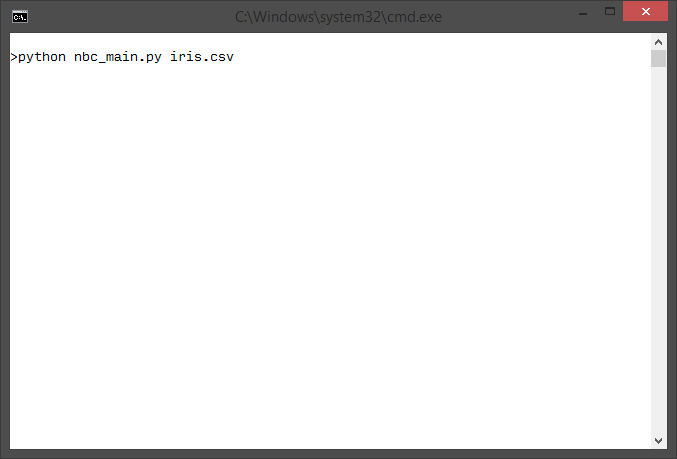
\includegraphics[width = \columnwidth]{./assets/y03s01-syssoft-term-paper-01-p01.png}
							\caption{}
							\label{subfig:nbc-usage}
						\end{subfigure}\quad%
						\begin{subfigure}[b]{0.5\columnwidth - 0.5em}
							\centering
							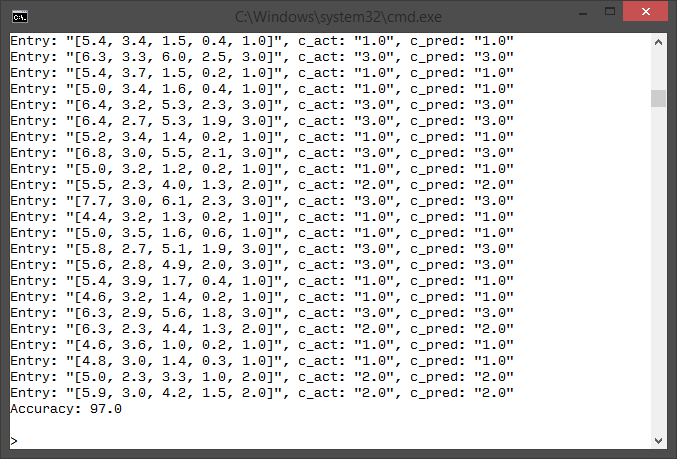
\includegraphics[width = \columnwidth]{./assets/y03s01-syssoft-term-paper-01-p02.png}
							\caption{}
							\label{subfig:nbc-res-01}
						\end{subfigure}
						\begin{subfigure}[b]{0.5\columnwidth - 0.5em}
							\centering
							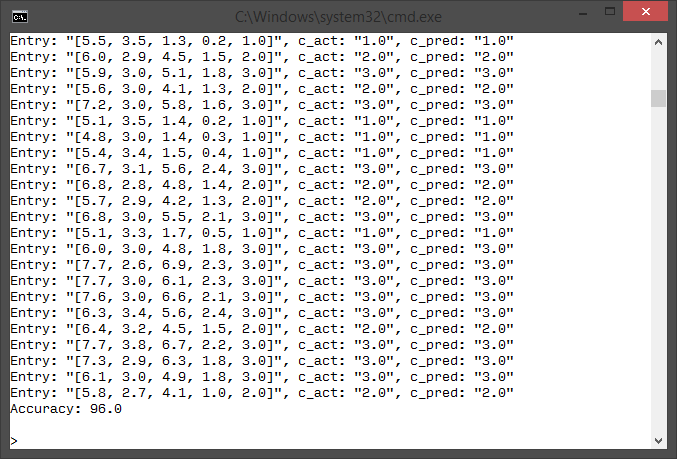
\includegraphics[width = \columnwidth]{./assets/y03s01-syssoft-term-paper-01-p03.png}
							\caption{}
							\label{subfig:nbc-res-02}
						\end{subfigure}\quad%
						\begin{subfigure}[b]{0.5\columnwidth - 0.5em}
							\centering
							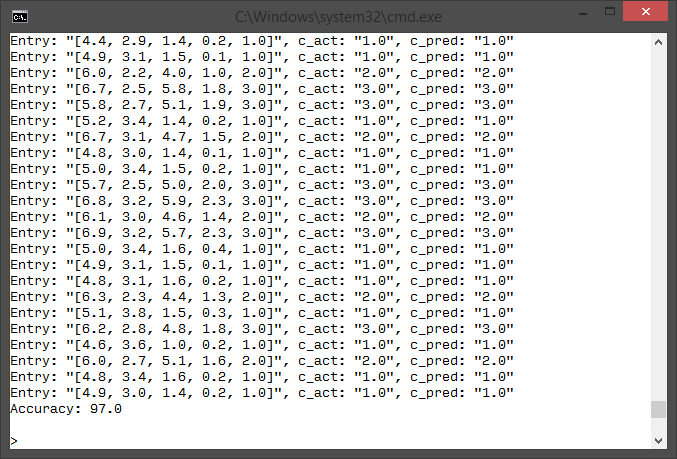
\includegraphics[width = \columnwidth]{./assets/y03s01-syssoft-term-paper-01-p04.png}
							\caption{}
							\label{subfig:nbc-res-03}
						\end{subfigure}
						\caption{Процес тестування розробленої реалізації: \subref{subfig:nbc-usage}~— запуск програми, \subref{subfig:nbc-res-01}–\subref{subfig:nbc-res-03}~— результати класифікації}
						\label{fig:nbc-testing}
					\end{figure}

					Результат тестування показав працездатність програми і~високий рівень точності на~тестовому наборі даних у~3~проведених експериментах: \SI{97.0}{\percent}, \SI{96.0}{\percent} та~\SI{97.0}{\percent} відповідно.

	\newpage
	\addsec{Висновки}

		У~процесі виконання даної курсової роботи була створена програмна реалізація наївного баєсового класифікатора для~класифікації неперервних числових даних. Для~розробки реалізації була використана мова програмування~\textenglish{Python} і~засоби її~стандартної бібліотеки: модулі~\modulename{argparse}, \modulename{csv}, \modulename{random}. Виконуючи дану курсову роботу, я~ознайомився із~задачею класифікації даних, поняттям класифікатора і~теоретичними відомостями про~наївний баєсів класифікатор. Я~дізнався про~поняття моделі подій, а~також ознайомився з~процесом оцінки параметрів імовірнісної моделі баєсового класифікатора. Крім того, я~навчився реалізовувати математичне представлення класифікатора на~практиці, а~також набув навичок розробки і~відладки модулів, написаних на~мові програмування~\textenglish{Python}.

	\newpage
	\printbibliography

	% \newcommand*{\appendixmore}{%
	% 	\renewcommand*{\sectionformat}{%
	% 		\appendixname~\thesection\autodot\enskip%
	% 	}
	% 	\renewcommand*{\sectionmarkformat}{%
	% 		\appendixname~\thesection\autodot\enskip%
	% 	}
	% }
	\newpage
	% \appendix
	\appsection{Початковий код}
		\begin{listingpython}[toprule = 0pt, bottomrule = 0pt]{Файл~\filename{nbc\_main.py}}{lst:nbc-main-py}
# This is a Naive Bayes Classifier implementation in Python
# written by Vlad Klokun and Igor Rabin
#
# Inputs: a CSV data file that contains training data
# Does: analyzes given CSV training file according to the Naive Bayes Classifier algorithm, generates random data and then makes a prediction about it
#
# Assumes a Gaussian Distribution

#!/usr/bin/env/ python3

import csv # reading CSV files
import random # list shuffling
import math # exp, pow etc

# Loads a valid CSV file containing floating-point training data into memory
# Input: a filename of a training file in CSV format
# Output: a dataset in form of a list of floats
def load_training(filename):
    with open(filename) as file:
        # ignore all lines which start with '#'
        reader = csv.reader(row for row in file if not row.startswith('#'))
        dataset = []
        for row in reader:
            # comprehend each line as a list of floats and append it to the dataset
            dataset.append([float(x) for x in row])

    return dataset

# split_dataset() splits a given dataset into 'training' and 'test' datasets to test the algorithm
# Inputs: a dataset (list), split_ratio (float)
# Outputs: a tuple of: dataset_train --- training dataset (list), dataset_test --- dataset (list)
def split_dataset(dataset, ratio):
    dataset_shuffled = dataset
    random.shuffle(dataset_shuffled)
    dataset_train = dataset_shuffled[:int(len(dataset_shuffled) * ratio)]
    dataset_test = dataset_shuffled[int(len(dataset_shuffled) * ratio):]

    return dataset_train, dataset_test

# Separate entries by class. Assumes that class is the last parameter
# Input: dataset
# Output: dictionary with class as key and matching entries as values
def separate_by_class(dataset):
    separated = {}
    for entry in dataset:
        # if entry with a given label is not yet in the dictionary, add it
        if entry[-1] not in separated:
            separated[entry[-1]] = []

        separated[entry[-1]].append(entry)

    return separated

# calc_mean(): Calculates mean value of a given sequence
# Inputs: seq — a sequence of numbers
# Outputs: a mean value of the sequence (float)
def calc_mean(seq):
    return sum(seq) / len(seq)

# calc_variance(): Calculates variance of a given sequence
# Input: seq --- a sequence of numbers
# Output: variance --- variance value (sigma^2) computed using n - 1 estimator
def calc_variance(seq):
    if len(seq) == 1:
        return 0
    # expected value
    mean = calc_mean(seq)
    # the variance of the set assuming all values are equally likely
    # use n - 1 estimator
    variance = sum([pow(x - mean, 2) for x in seq]) / (len(seq) - 1)
    # return math.sqrt(variance)
    return variance

# summarize(): summarizes every attribute in a dataset with their probabilistic properties: mean and variance. Makes no distiction based on class variables. returns a list of tuples which contain mean and variance values for respective attributes
# Input: dataset --- a list containing a dataset
# Output: summaries --- a list of tuples with statistical properties for each attribute in form of (mean, variance)
def summarize(dataset):
    summaries = []
    for attribute in zip(*dataset):
        summaries.append((calc_mean(attribute), calc_variance(attribute)))

    # removes summary for last column — class
    del summaries[-1]
    return summaries

# summarize_by_class(): summarizes every attribute in a dataset with their probabilistic properties: mean and variance. Unlike summarize(), the attributes are summarized on a per-class basis. Returns a list of tuples which contain mean and variance values for respective attributes belonging to certain classes.
# Input: dataset --- a dataset
# Output: summaries --- a dictionary with class variables as keys and statistical summaries of attributes as values
def summarize_by_class(dataset):
    separated = separate_by_class(dataset)
    summaries = {}
    for class_value, data in separated.items():
        summaries[class_value] = summarize(data)

    return summaries

# calculate_probability(): calculates probability of a given value X belonging to a certain class, assuming Gaussian distribution and passed mean and variance values
# Input 1: x --- value to be tested for belonging to a certain class
# Input 2: mean --- mean value for an attribute which the value is tested against
# Input 2: variance --- variance value for an attribute which the value is tested against
def calculate_probability(x, mean, variance):
    # if variance = 0 attribute values are the same and testing doesn't really make sense
    if variance == 0:
        return 0
    exp = math.exp( (-math.pow(x - mean, 2) ) / (2 * variance) )
    return (1 / math.sqrt(2 * math.pi * variance)) * exp

# calc_class_probability(): calculates probabilities of given input vector belonging to every class
# Input 1: summaries --- list of statistical summaries for every class
# Input 2: input_vector --- an entry to be classified
# Output: probabilities --- a dictionary containing probabilities of an entry belonging to each class
def calc_class_probability(summaries, input_vector):
    probabilities = {}
    for class_value, summaries in summaries.items():
        probabilities[class_value] = 1
        for (mean, variance), x in zip(summaries, input_vector):
            probabilities[class_value] *= calculate_probability(x, mean, variance)

    return probabilities

# predict(): predicts the class of a given entry
# Input 1: summaries --- list of statistical summaries for every class
# Input 2: input_vector --- an entry to be classified
# Output 1: key value of a class to which given entry most possibly belongs
def predict(summaries, input_vector):
    probabilities = calc_class_probability(summaries, input_vector)
    # get key with max value
    return max(probabilities, key = probabilities.get)

# predict_dataset(): makes predictions for a whole given dataset
# Input 1: summaries --- list of statistical summaries for every class
# Input 2: dataset --- a dataset to be classified
# Output 1: predictions --- a list of class values, to which entries are predicted to belong
def predict_dataset(summaries, dataset):
    predictions = []
    for entry in dataset:
        predictions.append(predict(summaries, entry))

    return predictions

# compute_accuracy(): computes accuracy of predictions given the dataset with known-good class variables
# Input 1: dataset --- a dataset with known-good classification
# Input 2: predictions --- a list of predictions made by the Native Bayes Classifier
# Output 1: accuracy in %
def compute_accuracy(dataset, predictions):
    correct = 0
    for entry, prediction in zip(dataset, predictions):
        # c_act --- actual known-good class, c_pred --- class predicted by Naive Bayes Classifier
        print('Entry: "{}", c_act: "{}", c_pred: "{}"'.format(entry, entry[-1], prediction))
        if entry[-1] == prediction:
            correct += 1

    return (correct / len(dataset)) * 100.0

		\end{listingpython}

		\begin{listingpython}[toprule = 0pt, bottomrule = 0pt]{Файл~\filename{nbc.py}}{lst:nbc-py}
#!/usr/bin/env python3

import argparse
from nbc import *

def main(args):
    dataset = load_training(args.input)
    dataset_train, dataset_test = split_dataset(dataset, 1/3) # split dataset 1 / 3

    summaries = summarize_by_class(dataset_test)
    predictions = predict_dataset(summaries, dataset_test)
    acc = compute_accuracy(dataset_test, predictions)
    print('Accuracy: {}'.format(acc))

if __name__ == '__main__':
    parser = argparse.ArgumentParser(description = 'An implementation of Gaussian Naive Bayes Classifier in Python using stdlib facilities. Reads a CSV file containing floats.')

    # Parse CSV dataset file
    parser.add_argument('input', help = 'Path to input file')
    
    args = parser.parse_args()

    main(args)
		\end{listingpython}

	\newpage
	\appsection{Набір даних~«Іриси Фішера»}
		\begin{listingpython}[toprule = 0pt, bottomrule = 0pt]{Файл~\filename{iris.csv}}{lst:iris-csv}
5.1,3.5,1.4,0.2,1
4.9,3.0,1.4,0.2,1
4.7,3.2,1.3,0.2,1
4.6,3.1,1.5,0.2,1
5.0,3.6,1.4,0.2,1
5.4,3.9,1.7,0.4,1
4.6,3.4,1.4,0.3,1
5.0,3.4,1.5,0.2,1
4.4,2.9,1.4,0.2,1
4.9,3.1,1.5,0.1,1
5.4,3.7,1.5,0.2,1
4.8,3.4,1.6,0.2,1
4.8,3.0,1.4,0.1,1
4.3,3.0,1.1,0.1,1
5.8,4.0,1.2,0.2,1
5.7,4.4,1.5,0.4,1
5.4,3.9,1.3,0.4,1
5.1,3.5,1.4,0.3,1
5.7,3.8,1.7,0.3,1
5.1,3.8,1.5,0.3,1
5.4,3.4,1.7,0.2,1
5.1,3.7,1.5,0.4,1
4.6,3.6,1.0,0.2,1
5.1,3.3,1.7,0.5,1
4.8,3.4,1.9,0.2,1
5.0,3.0,1.6,0.2,1
5.0,3.4,1.6,0.4,1
5.2,3.5,1.5,0.2,1
5.2,3.4,1.4,0.2,1
4.7,3.2,1.6,0.2,1
4.8,3.1,1.6,0.2,1
5.4,3.4,1.5,0.4,1
5.2,4.1,1.5,0.1,1
5.5,4.2,1.4,0.2,1
4.9,3.1,1.5,0.1,1
5.0,3.2,1.2,0.2,1
5.5,3.5,1.3,0.2,1
4.9,3.1,1.5,0.1,1
4.4,3.0,1.3,0.2,1
5.1,3.4,1.5,0.2,1
5.0,3.5,1.3,0.3,1
4.5,2.3,1.3,0.3,1
4.4,3.2,1.3,0.2,1
5.0,3.5,1.6,0.6,1
5.1,3.8,1.9,0.4,1
4.8,3.0,1.4,0.3,1
5.1,3.8,1.6,0.2,1
4.6,3.2,1.4,0.2,1
5.3,3.7,1.5,0.2,1
5.0,3.3,1.4,0.2,1
7.0,3.2,4.7,1.4,2
6.4,3.2,4.5,1.5,2
6.9,3.1,4.9,1.5,2
5.5,2.3,4.0,1.3,2
6.5,2.8,4.6,1.5,2
5.7,2.8,4.5,1.3,2
6.3,3.3,4.7,1.6,2
4.9,2.4,3.3,1.0,2
6.6,2.9,4.6,1.3,2
5.2,2.7,3.9,1.4,2
5.0,2.0,3.5,1.0,2
5.9,3.0,4.2,1.5,2
6.0,2.2,4.0,1.0,2
6.1,2.9,4.7,1.4,2
5.6,2.9,3.6,1.3,2
6.7,3.1,4.4,1.4,2
5.6,3.0,4.5,1.5,2
5.8,2.7,4.1,1.0,2
6.2,2.2,4.5,1.5,2
5.6,2.5,3.9,1.1,2
5.9,3.2,4.8,1.8,2
6.1,2.8,4.0,1.3,2
6.3,2.5,4.9,1.5,2
6.1,2.8,4.7,1.2,2
6.4,2.9,4.3,1.3,2
6.6,3.0,4.4,1.4,2
6.8,2.8,4.8,1.4,2
6.7,3.0,5.0,1.7,2
6.0,2.9,4.5,1.5,2
5.7,2.6,3.5,1.0,2
5.5,2.4,3.8,1.1,2
5.5,2.4,3.7,1.0,2
5.8,2.7,3.9,1.2,2
6.0,2.7,5.1,1.6,2
5.4,3.0,4.5,1.5,2
6.0,3.4,4.5,1.6,2
6.7,3.1,4.7,1.5,2
6.3,2.3,4.4,1.3,2
5.6,3.0,4.1,1.3,2
5.5,2.5,4.0,1.3,2
5.5,2.6,4.4,1.2,2
6.1,3.0,4.6,1.4,2
5.8,2.6,4.0,1.2,2
5.0,2.3,3.3,1.0,2
5.6,2.7,4.2,1.3,2
5.7,3.0,4.2,1.2,2
5.7,2.9,4.2,1.3,2
6.2,2.9,4.3,1.3,2
5.1,2.5,3.0,1.1,2
5.7,2.8,4.1,1.3,2
6.3,3.3,6.0,2.5,3
5.8,2.7,5.1,1.9,3
7.1,3.0,5.9,2.1,3
6.3,2.9,5.6,1.8,3
6.5,3.0,5.8,2.2,3
7.6,3.0,6.6,2.1,3
4.9,2.5,4.5,1.7,3
7.3,2.9,6.3,1.8,3
6.7,2.5,5.8,1.8,3
7.2,3.6,6.1,2.5,3
6.5,3.2,5.1,2.0,3
6.4,2.7,5.3,1.9,3
6.8,3.0,5.5,2.1,3
5.7,2.5,5.0,2.0,3
5.8,2.8,5.1,2.4,3
6.4,3.2,5.3,2.3,3
6.5,3.0,5.5,1.8,3
7.7,3.8,6.7,2.2,3
7.7,2.6,6.9,2.3,3
6.0,2.2,5.0,1.5,3
6.9,3.2,5.7,2.3,3
5.6,2.8,4.9,2.0,3
7.7,2.8,6.7,2.0,3
6.3,2.7,4.9,1.8,3
6.7,3.3,5.7,2.1,3
7.2,3.2,6.0,1.8,3
6.2,2.8,4.8,1.8,3
6.1,3.0,4.9,1.8,3
6.4,2.8,5.6,2.1,3
7.2,3.0,5.8,1.6,3
7.4,2.8,6.1,1.9,3
7.9,3.8,6.4,2.0,3
6.4,2.8,5.6,2.2,3
6.3,2.8,5.1,1.5,3
6.1,2.6,5.6,1.4,3
7.7,3.0,6.1,2.3,3
6.3,3.4,5.6,2.4,3
6.4,3.1,5.5,1.8,3
6.0,3.0,4.8,1.8,3
6.9,3.1,5.4,2.1,3
6.7,3.1,5.6,2.4,3
6.9,3.1,5.1,2.3,3
5.8,2.7,5.1,1.9,3
6.8,3.2,5.9,2.3,3
6.7,3.3,5.7,2.5,3
6.7,3.0,5.2,2.3,3
6.3,2.5,5.0,1.9,3
6.5,3.0,5.2,2.0,3
6.2,3.4,5.4,2.3,3
5.9,3.0,5.1,1.8,3
		\end{listingpython}

\end{document}
